\documentclass{article}

\usepackage[english]{babel}
\usepackage[utf8]{inputenc}
\usepackage{amsmath}
\usepackage{graphicx}
\graphicspath{ {./images/} }
\begin{document}

\begin{titlepage}
\pagenumbering{gobble}
\addcontentsline{toc}{section}{Abstract}
\begin{center}
\vspace{1cm}
\huge
\textbf{My E-Gardener}

\LARGE
\vspace{.5cm}
IT-project with regard to our B.Sc in Software Engineering at the University of The Faroe Islands


\vspace{.5cm}
\textbf{Kristmund Ryggstein and Hergeir Winther Lognberg}\\
\vspace{.5cm}
\Large
\vspace{.5cm}
\pagebreak
\Large
\textbf{Abstract}
\end{center}
We were asked to do an it project using an Arduino Uno. We chose to to do an automated gardening system with it, because that is relevent for some work projects that are currently in progress on Sandoy, where we are from. Our ardunio project entails an automated system that waters, measures moisture, heat and light exposure. That is done by customizing an Arduino Uno which has a moisture-, heat and light sensor that does all our measurements. All the the data is then collected by the Arduino, and then sent to a Web Service via. a esp-05 wifi module. The Web Service receives the data, and presents it to the user. The user is registered with the Web Service, and can track his plant data through his registered user account, where he also can customize water input for the plant/s.

The service was devoloped in ASP.Net, which was a class we had prior to this one and we thought it would be a practical platform for developing a service centered around our E-gardening data.

The code uses a design pattern called Observer Pattern. It's function is to solve text\footnote{\url}

\begin{quote}
"one-to-many dependency between objects should be defined without making the objects tightly coupled.

It should be ensured that when one object changes state an open-ended number of dependent objects are updated automatically.

It should be possible that one object can notify an open-ended number of other objects."
\end{quote}

This means 

\vfill
\begin{center}
Náttúruvísindadeildin\\
Benadikt Joensen, Gunnar Restorff\\
University of the Faroe Islands\\
January 2019\\
\end{center}
\end{titlepage}
\pagenumbering{gobble}
\tableofcontents
\listoffigures
\listoftables
\pagebreak
\pagenumbering{gobble}
\begin{center}\section*{Acknowledgments}\end{center}
\addcontentsline{toc}{section}{Acknowledgments}

\pagebreak
\pagenumbering{arabic}
\section{Introduction}

As said our project is about a system that automates taking care of some vegetation of some kind, be it house plants, garden plants or even vegetative food. We have seen that the interest for growing vegetables in the Faroe Islands has been increased with initiatives such as "Eplafestivalurin", and "Veltan" which has received government funding. Veltan's goal is to grow and sell Faroese vegetables and fruits, and give everyone a place with resources, so that they are able to grow their own things.


Veltan's coincides well with UN's campaign "Goal 2:Zero Targets" which is trying to change and optimize the world's agriculture in hopes to feed the 815 people that are undernourished today and the additional 2 billions people expected to be malnourished in 2050\footnote{https://www.un.org/sustainabledevelopment/hunger/}. Agriculture derived foot is more energy efficient than meat farming\footnote{•} and contributes less pollution, because energy consumption is wasted the higher up we go through the food chain, so optimizing our production in agricultural farming would be the best way to achieve UN's goal.

Taking care of vegetation is task that is easy to forget which is why we thought that it was a process that was convenient to automate, and a cheap automated gardening system for the everyday household might also help with UN's goals, as it would mean that everyone had easy and cheap tool to help them with growing their crops.

\section{Materials}
The Arduino Uno, TMP36GZ heat sensor, resistors and the cables which we use in this project, was provided by the one responsible by the course. We used at the start a FC28 moisture sensor, but it generally uses DC current which means that because of electrolysis in the soil it corrodes fairly quickly and alters the soil composition, which could potentially damage the plant and lead to tainted readings. We changed it to use an AC pulse, but we decided to opt for Capacitive Soil Moisture Sensor V1.2 that is Corrosion Resistant.


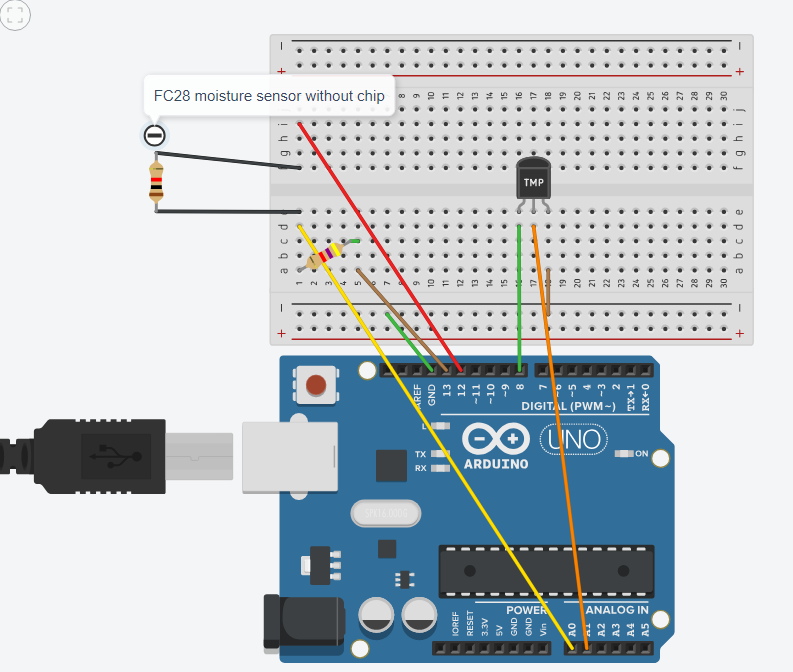
\includegraphics[scale = 0.50]{FC-28-Diagram.PNG}


We started testing the project with the FC28 moisture until we received the new sensor.

\section{Code}

\subsection{Method}

Our intention was to use the arduino to induce an alternating current through the sensor. To simplify things, we cirqumvented the cirquit of FC-28 such that we connected directly to the pins on the sensor. To alternate the current, we first emmit 5v from pin 12 and set pin 13 to low (0v) for 1 ms then we take a reading through the analog pin A0. Then we flip the pin 12 and 13 ( 5v from pin 13 ) for the same amount of time. This should somewhat remidy the problems of electrolysis by shifting the ions back and forth between the pins instead of just one way.

The resistor in the cirquit helps increase the amount of current entering the analog sensor. Without it about half the current would go in the pin 13 when the measurement occurst. By changing the resistor we are thereby able to steer the range of current entering the analog input.


\section{Attachments}
\begin{figure}
  \centering
      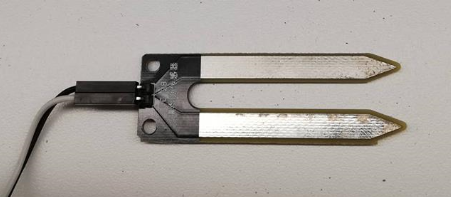
\includegraphics{fc-28-corrosion}
  \caption{Corroded fc-28 after moderate use.}
\end{figure}


\pagebreak
\pagenumbering{gobble}
\addcontentsline{toc}{section}{References}
\bibliographystyle{ieeetr}
\nocite{*}
% \bibliography{biblio.bib}
% change the file name to line up with your bibtex file


\end{document}